\chapter{Circuit design}
This chapter describe the design methodology in implementing analog blocks used in third order $\Delta\Sigma$ modulator, and also address the issues involving the design of the modulator. 

Moreover the procedure to obtain the final transistor dimensions were based on the $gm/I_D$ methodology and on iterative simulations, since the equations used in the SPICE level 1 are not accurate. 

\section{Switched-Capacitor Circuits}

As discussed in chapter \ref{architecture} resistors occupy huge space in a layout and they are also the sources of noises, which makes them unattractive to use in integrated circuits. A switched capacitor circuit can be used to emulate the behaviour of a resistor by a capacitor in and out of the circuit. Figure \ref{fig:switched_cap} depict a switch-capacitor circuit, where \textit{$V_1$} and \textit{$V_2$} are two dc voltage sources. The clock periods $\phi_1$ and $\phi_2$ are a pair of overlapping clocks, which means that the capacitor $C_1$ is charged to $V_1$ and then $V_2$ during each clock period. This charge transfer is repeated every clock period with a clock period of $T_s$. Thus, the average current is given by the charge moved in one clock period\cite{Johns}:  

\begin{equation}\label{sw_res}
    I_{avg} = \frac{C_1(V_1 - V_2)}{T_s}
\end{equation}

\begin{figure}[h]
\begin{subfigure}[c]{0.4\linewidth}
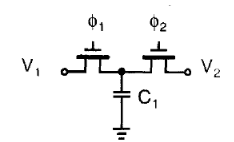
\includegraphics[width=\linewidth]{images/switched_cap_res.png}
\caption{Switched-capacitor circuit}
\label{fig:switched_cap}
\end{subfigure}
\hfill
\begin{subfigure}[c]{0.3\linewidth}
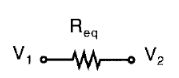
\includegraphics[width=\linewidth]{images/res.png}
\caption{Resistor equivalent}
\label{fig:resistor}
\end{subfigure}

\caption{Resistor equivalence of switched capacitor capacitor}
\end{figure}

From the equivalent resistor circuit shown in figure \ref{fig:resistor}, we have that the current through the resistor is:

\begin{equation}\label{eq}
    I = \frac{V_1-V_2}{R_{eq}}
\end{equation}

Comparing equations \ref{sw_res} and \ref{eq}, we see that the average current through the SC circuit will be equal to the resistor circuit if:

\begin{equation}
    R_{eq} = \frac{T_s}{C_1} = \frac{1}{C_1f_s}
\end{equation}

A disadvantage is that the switches are implemented using transistors, and their non-idealities can degrade the SC circuit performance. 

\section{Switched-Capacitor Integrators}
A differential switched-capacitor integrator circuit is shown in Fig. \ref{fig:DT_integrator}. It is known for its insensitive to parasitic capacitance of the sampling capacitor ($C_s$). The operation of the SC integrator can be explained by examining the charges on the capacitors on each clock phase. For simplicity we will only look at the top half circuit, since the bottom one has the same operation. It is assumed that the initial voltage stored in $C_f$ is zero. Switches \textit{S1} and \textit{S3} are closed during phase $\Phi_1$, while the others are closed during phase $\Phi_2$. Note that $\Phi_1$ and $\Phi_2$ are two non-overlapping phases. When \textit{S1} and \textit{S3} are closed, the input source charges the capacitor $C_s$ to a initial charge of $C_sV_{IN}$. During phase $\Phi_2$ switches \textit{S2} and \textit{S4} are closed. Thus the input is disconnected from the circuit, and the bottom plate of capacitor $C_s$ is connected to ground. Therefore the charge stored on the capacitor $C_s$ is transferred to the capacitor $C_f$. Then when phase $\Phi_1$ is active again the input voltage charge $C_s$ with a new sample. Then during phase $\Phi_2$, the charge from the new sample is transferred to the capacitor $C_f$ where it accumulates with the previous charge from the first operation. The integrator corresponds to a non-inverting one, and the transfer function is given by equation \ref{transfer_integrator}.

\begin{figure}[h]
\centering
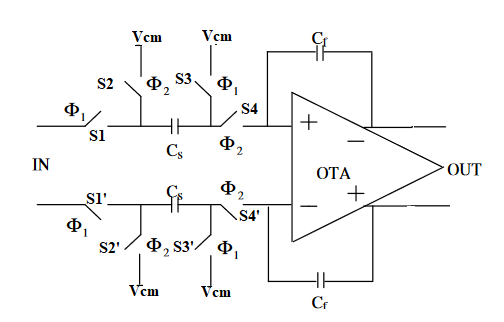
\includegraphics[scale=0.8]{images/DT_integrator.png}
\caption{Parasitic-insensitive integrator}
\label{fig:DT_integrator}
\end{figure}


\subsection{Channel Charge Injection and Bottom-Plate Sampling}
Charge injection can be understood using the circuit in Fig. \ref{fig:charge_injection}. When the MOSFET switch is \textit{on} and $V_{DS}$ is small, there is a charge present in the inversion layer called channel charge $Q_{ch}$. When the MOSFET turns of, this charge is injected onto the capacitor $C_{load}$ and into $V_{in}$. Since $V_{in}$ is assumed to be a low-impedance, source driven node, the injected charge has no effect on this node. However, the charge injected onto $C_{load}$ results in a change in voltage across it, introducing an error in reading the correct input signal. 

\begin{figure}[H]
\centering
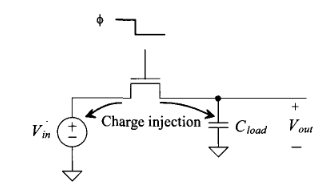
\includegraphics[scale=0.9]{images/charge_injection.png}
\caption{Charge injection in a sampling circuit}
\label{fig:charge_injection}
\end{figure}

Although charge injection mechanism is complex to characterize, many techniques have been used to minimize its effect. One being bottom-plate sampling technique\cite{Barker} which is employed to make charge injection of switches independent of the input signal. Figure \ref{fig:bottom_sampling} shows the integrator again, but now with delayed phases $\Phi_{1d}$ and $\Phi_{2d}$ with respect to phases $\Phi_1$ and $\Phi_2$ respectively. Switches \textit{S3} and \textit{S4} are turned off slightly before switches \textit{S1} and \textit{S2}, so that $C_s$ sees a high impedance. Thus, the charge injection introduced by switches \textit{S1} and \textit{S3} flows towards the low-impedance source node and almost no charge is accumulated onto sampling capacitor $C_s$.

\begin{figure}[ht]
\centering
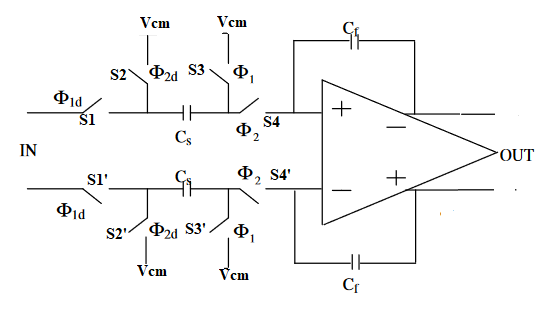
\includegraphics[scale=0.7]{images/DT_integrator_delayed.png}
\caption{Integrator with bottom-sampling technique}
\label{fig:bottom_sampling}
\end{figure}

\subsection{Correlated Double Sampling}

Correlated double sampling (CDS) technique was first introduced by White, Lampe, Biaha and Mack \cite{cds} as a technique for removal of switching transients and elimination of the Nyquist noise. What is more interesting is that it can be used to attenuate errors due to flicker noise $1/f$, finite offset voltage and finite opamp gain \cite{corr}. The technique is only used on the first integrator since the noise contribution is most critical in it. The noise contribution in the subsequent integrators are small, since the noise will be significantly attenuated as discussed in the feasibility study. 

We will use a simple SC integrator depict in Fig. \ref{fig:cds} to illustrate how the CDS technique works. During $\phi_1$, the capacitor $C_2'$ samples the input offset voltage of the opamp. Then $C_2'$ is connected in series with the opamp's inverting input during phase $\phi_2$. The error from the opamp gets subtracted from the one stored in $C_2'$, thus minimizing it. For a differential SC integrator a symmetrical circuit of the one shown in \ref{fig:cds} is connected to the non-inverting input.  

\begin{figure}[ht]
\centering
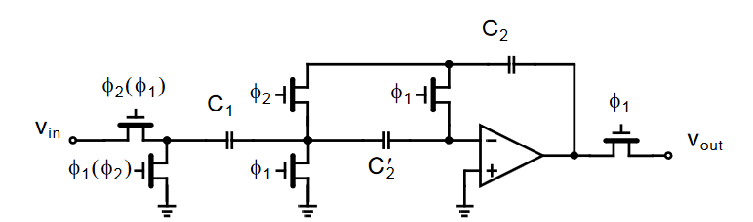
\includegraphics[width=\textwidth]{images/cds.png}
\caption{Simple SC integrator using CDS technique \cite{Johns} }
\label{fig:cds}
\end{figure}

Another thing to note is that CDS will square the effective gain to the opamp due the extra capacitors, so the open-loop gain of the OTA for integrator will get relaxed, as seen in table \ref{spec_ota}, but at the expanse of bigger area. The resulting schematic of integrator 1 is shown in Fig. ?? 


\section{Switches}
Sampling switches is one of the most fundamentals analog blocks of ADC operating on discrete-time. An ideal switch is just short circuit when it is \textit{on} and an open circuit when it is \textit{off}. In other words when the switch is \textit{on} there should be zero resistance, and when the switch is \textit{off} there should be an infinity resistance. But as discussed in section \ref{on-resistance}, these values are not feasible. Therefore designing the switches with adequate on-resistances without degrading the performance is a crucial part of designing a data converter. 

The commonly used switch implementations are: a NMOS transistor, a PMOS transistor or a transmission gate (TG). The on-resistance of a MOSFET depends on the input signal, as given in \cite{Allen}, and rewritten in expression \ref{R_on}:

\begin{equation}\label{R_on}
    R_{on} = \frac{1}{\mu C_{ox}\frac{W}{L}(V_{GS} - V_T)}
\end{equation}

From the expression we get that the time-constant increases for more positive NMOS or negative PMOS inputs. Designing a switch with large enough input swing capability is a challenge in low-voltage application. The reason being that as the technology scales, the supply voltage scales down much faster than the threshold voltage of a transistor. For a NMOS the operation is restricted to a input swing lower than $V_{DD} - V_{thn}$, and for PMOS the swing must be greater than $V_{thp}$. 

Transmission gate is a technique that can be used to accommodate greater swings \cite{Barker}. It consists of a PMOS in parallel with a NMOS transistor as shown in Fig. \ref{fig:TG_switch}. The disadvantage of such switch is to have extra circuit to implement the complementary clocks, but it is a small price to pay for an improvement as good as rail-to.rail swing across the switch.     

\begin{figure}[h]
\centering
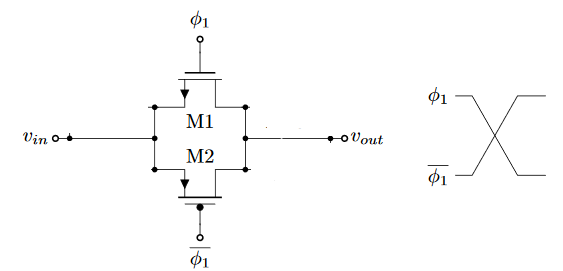
\includegraphics[scale=0.7]{images/TG_switch.png}
\caption{Circuit implementation of a TG switch}
\label{fig:TG_switch}
\end{figure}

After choosing the topology for the switch, the dimensions of the transistors were found. Using equation \ref{R_on} and Fig. \ref{fig:TG_switch} we get that: $V_{GS} = \phi_1 - v_{in}$, where $\phi_1$ is $V_{DD}=1.8V$ when it is \textit{on} and 0V when it is \textit{off}. After completing a simulation it was found out that the on-resistance for the resistors were too high. We cannot change the swing of the input voltage $V_{in}$, since it is given by the system. The options were either to increase the dimension $\frac{W}{L}$ or increase the gate voltage $\phi$ when it is high. Since we want to keep the dimensions as small as possible, we increased the gate voltage. In order to increase the supply voltage $V_{DD}$ a charge pump was used \cite{charge_pump}. It is a Dc-to-Dc converter that can take a a DC source from one level to another. In our case it was found out that doubling $V_{DD}$ was sufficient enough to get the on-resistance in the range we wanted. The charge pump was not implemented on circuit level, instead an ideal DC source was used to mimic the behaviour of the charge pump. Finally we used a level-shifter \cite{William} to translate signals from one voltage domain to another, namely $[0,V_{DD}]$ to $[0,2V_{DD}]$. 

The switches were chosen to have minimum dimensions. Moreover the PMOS transistors were chosen to be three times bigger than the NMOS transistors to account lower mobility.. for varying switching time, and make the on-resistance more independent of the input voltage. The final dimensions for the switches of integrator 1 are listed in table \ref{R_on_1} and for integrator 2,3 and the sum block in tables \ref{R_on_2}, \ref{R_on_3} and \ref{R_on_sum} respectively in appendix \ref{app:on_resistance}. Compared with table \ref{on-resistance} we see that the on-resistance of the switches of the integrators approximately meets the specifications. It does not matter if the on-resistances varies with a couple of $\Omega s$ since it only affect the performance to a small degree. 

\begin{table}[ht]
\centering
\caption{Switch transistors' dimensions and resistances of integrator 1}
\label{R_on_1}
\begin{tabular}{|l|l|l|l|}
\hline
Switch & PMOS( W/L)$\mu m$ & NMOS( W/L)$\mu m$ & $R_{ON} (\Omega)$   \\ \hline
I23    & 13.5/0.55  & 4.5/0.55   & 904.9 \\ \hline
I9     & 14.7/0.55  & 4.9/0.55   & 907.2 \\ \hline
I18    & 13.2/0.55  & 4.4/0.55   & 892.2 \\ \hline
I20    & 11.7/0.55  & 3.9/0.55   & 903.8 \\ \hline
\end{tabular}
\end{table}

\section{Operational Tranceconductance Amplifier}

Operational tranceconductance amplifier (OTA) is the most important component of integrators in the $\Delta\Sigma$ modulator. Its specifications determine the performance of the integrator, thus of the whole modulator. Selection of topology for the OTAs and the design procedure to meet the specifications given by table \ref{spec_ota} will be discussed in the subsequent sections. 

\subsection{Selection of topology}
There are many architecture to choose from when designing a OTA, and they can be classified into two categories: single-stage and two-stage OTAs. In the single-stage category there are especially two architectures which are common to choose for low voltage/power operation: telescopic cascode and folded cascode. The conventional two-stage OTA is the miller configuration which commonly needs a class AB stage to enhance its speed \cite{two_stage_1},\cite{two_stage_2}. Table \ref{comparisom_OTA} compare the three OTAs in terms of power consummation, output-swing and speed.

\begin{table}[h]
\centering
\caption{Comparison between folded, telescopic and two-stage amplifiers\cite{Razavi}}
\label{comparisom_OTA}
\begin{tabular}{|l|l|l|l|}
\hline
Topology           & \begin{tabular}[c]{@{}l@{}}Power\\ Consumption\end{tabular} & \begin{tabular}[c]{@{}l@{}}Output\\ Swing\end{tabular} & Speed  \\ \hline
Folded Cascode     & Medium                                                      & Medium                                                 & Medium \\ \hline
Telescopic Cascode & Low                                                         & Low                                                    & High   \\ \hline
Two-stage          & High                                                        & High                                                   & Low    \\ \hline
\end{tabular}
\end{table}

The two-stage amplifier has high power consumption due to the compensation capacitors which inevitably end up consuming a considerable amount of current. Single-stage amplifiers offers good self compensation, thus they do not need extra capacitors resulting in lower power consumption. Moreover it has a lower dominant pole than single-stage amplifiers, hence it is difficult to use in high frequency applications. Keeping all these aspects in mind, the single-stage amplifiers were chosen to be analyzed more. 

The selection between folded cascode and telescopic cascode depends on the performance requirements. The topologies have somewhat similar characteristics with both having gain in medium ranges. Note that the folded cascode has higher voltage output-swing than the telescopic cascode due to less number of transistors stacked in the output branch of the folded cascode. However higher voltage swings means higher power consumption, lower voltage gain, lower pole frequencies and higher noise. Another advantage with folded cascode compared to telescopic cascode is that the input and output can be short together, and thereby relax the requirement of input common mode range (\textit{ICMR}). Since the gain requirement were low and the voltage output swing was high as seen in table \ref{spec_ota}, the folded cascode was chosen to be the most suitable among the two architectures.

\subsection{Single ended vs fully differential output }
In practice, fully differential output is used because it has many advantages over single ended \cite{Johns}. Some being:

$\bullet$ \textbf{Larger voltage output swing}: since the fully differential has twice as many output as the single ended one, the voltage output swing is almost double in magnitude. 

$\bullet$ \textbf{Higher SNR}: Since the voltage output swing is large we get a higher signal-to-noise ratio (SNR). The signal output power becomes four times bigger because of twice the output voltage, also the noise power is doubled. Hence we get a overall 3dB improvement in SNR or 0.5 bit improvement in effective number of bits (ENOB).

$\bullet$ \textbf{Better noise rejection}: It is less susceptibility to common mode noise.

One important thing to note with fully differential circuits is that they need additional circuit to keep the output common mode level stable i.e. a common mode feedback circuit is needed, which we will discuss later. This additional circuit causes larger area and higher power consumption compared to single ended topology\cite{Allen}. 

\subsection{The $g_m/I_D$ methodology}

With the emergence of advanced fabric processes the transistor dimensions have reduced drastically. As a consequence the traditional long-channel equations employed in the analog design were no longer producing desired results. In order to treat this inconvenience a new methodology was introduced by F. Silveria, D. Flandre and P. G. A. Jespers \cite{gm_id_1}. The method exploits the relationship between the ratio of the tranceconductance $g_m$ over dc drain current $I_D$ and the normalized drain current $I' = I_D/W$. It uses this relationship to determine the transistor dimensions to satisfy specifications like the GBW, low power, gain, etc. The $g_m/I_D$ ratio can be obtained by characterization of the process of the PMOS and NMOS transistors. Some of the key elements with the $g_m/I_D$  based design are described as follows\cite{gm_id_1},\cite{gm_id_2}:

$\bullet$ This method characterizes the performance of a transistor in all regions of operation. The curve generated for a particular process of a transistor is continuous and there are no transition in equations from various regions of operation, as it would be in the conventional long-channel equations. Thus we can freely select the device operation as per our needs. 

$\bullet$ With the generated curve one can easily derive the transistor dimensions meeting the specifications, as we will see later. 

$\bullet$ The amount of iteration in designing complex analog circuits is drastically reduced. The method gives a complete characterization of the technology, which involving take into account the parasitic influencing the device. Thus eliminating the approximate equation used to determine the device behaviour and improving the time used to design the circuits. 

\subsection{Design procedure of OTA}

The selected folded cascode architecture is shown in Fig. \ref{fig:folded_ota_design} showing the currents flowing through the different branches. The input pairs is PMOS differential pair. The flicker noise is less in a PMOS transistor, since its mobility is lower than of NMOS transistor\cite{Johns}. From the slew-rate and load capacitance ($C_L$) listed in table \ref{spec_ota} the bias current $I_1$ can be determined:

\begin{equation}\label{I_1}
    I_1 \geq SR*C_L
\end{equation}

As a rule of thumb, the load current $I_2$ should be in the range to keep all the transistors in saturation\cite{Razavi}:

\begin{equation}\label{I_2}
    1.2I_1<I_2<2I_1
\end{equation}

Thus making $I_3$ equal to:

\begin{equation}\label{I_3}
    I_3 = \frac{I_1}{2} + I_2
\end{equation}

\begin{figure}[h]
\centering
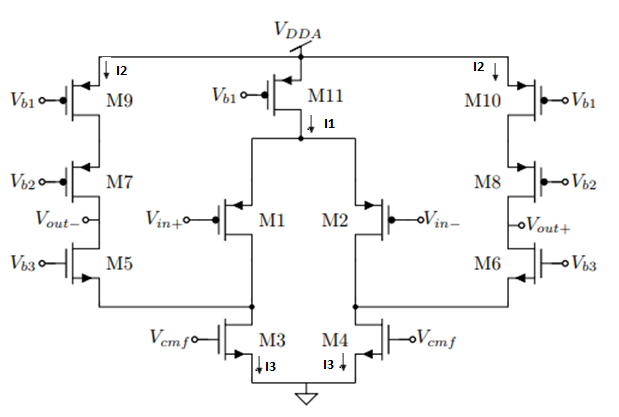
\includegraphics[scale = 0.8]{images/folded_cascode.png}
\caption{Folded cascode architecture with the current $I_1$, $I_2$ and $I_3$ flowing in different branches \cite{Grey}}
\label{fig:folded_ota_design}
\end{figure}

Tranceconductance of the circuit is given by GBW and $C_L$ as follows:

\begin{equation}
    gm_1 = GBW\cdot2\pi\cdot C_L
\end{equation}

The resulting bias currents and the tranceconductance of the circuit of OTA 1, 2 and 3 are listed in \ref{step_1}. These parameters can be used with the $g_m/I_D$ methodology to find the dimensions of the input transistors $M_1$ and $M_2$, as it will be described in the next section. 

\begin{table}[h]
\centering
\caption{The tranceconductance and bias current of OTA 1, 2 and 3}
\label{step_1}
\begin{tabular}{|l|l|l|}
\hline
OTA & $gm_1[\mu S]$ & $I_1[\mu A]$ \\ \hline
1   & 0.85  & 100  \\ \hline
2   & 0.15  & 20   \\ \hline
3   & 0.06   & 10   \\ \hline
\end{tabular}
\end{table}

\subsection{Obtaining transistor dimensions using $g_m/I_D$ methodology}

Using the design flow depict in Fig.\ref{design_slow} the procedure to find the dimensions of the transistors can be explained. The $g_m$ and $I_D$ is the tranceconductance and the drain current through a transistor respectively. 

\begin{figure}[H]
\centering
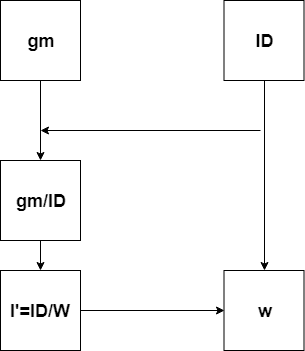
\includegraphics[scale = 0.45]{images/design_flow.png}
\caption{Design flow}
\label{design_slow}
\end{figure}

First step in the device characterization is to generate the plot of $g_m/I_D$ vs $I_D/W$. Figure
\ref{pmos_setup} shows a PMOS setup in cadence which is used to generate the plot. In a similar manner a NMOS transistor is setup to obtain the same plot. For this simulation transistor dimensions of $\frac{W}{L} = \frac{5\mu}{0.7\mu}$ is chosen. A comparison between the values of PMOS and NMOS transistors is shown in Fig. \ref{fig:comp_pmos_nmos}.

For illustrative purpose we will find the dimensions of transistor $M_1$ of OTA 1 and the design flow in Fig. \ref{design_slow} to get an insight on how the $g_m/I_D$ method works. From table \ref{step_1} we have that the $gm_1 = 0.85\mu S$ and the drain current through the transistor is given by:

\begin{equation}
    I_{M1} = \frac{I_1}{2} = 50\mu A
\end{equation}

which gives us:

\begin{equation}\label{gm_ID}
   gm_1/I_{M1} = 17 
\end{equation}



\begin{figure}[H]
\centering
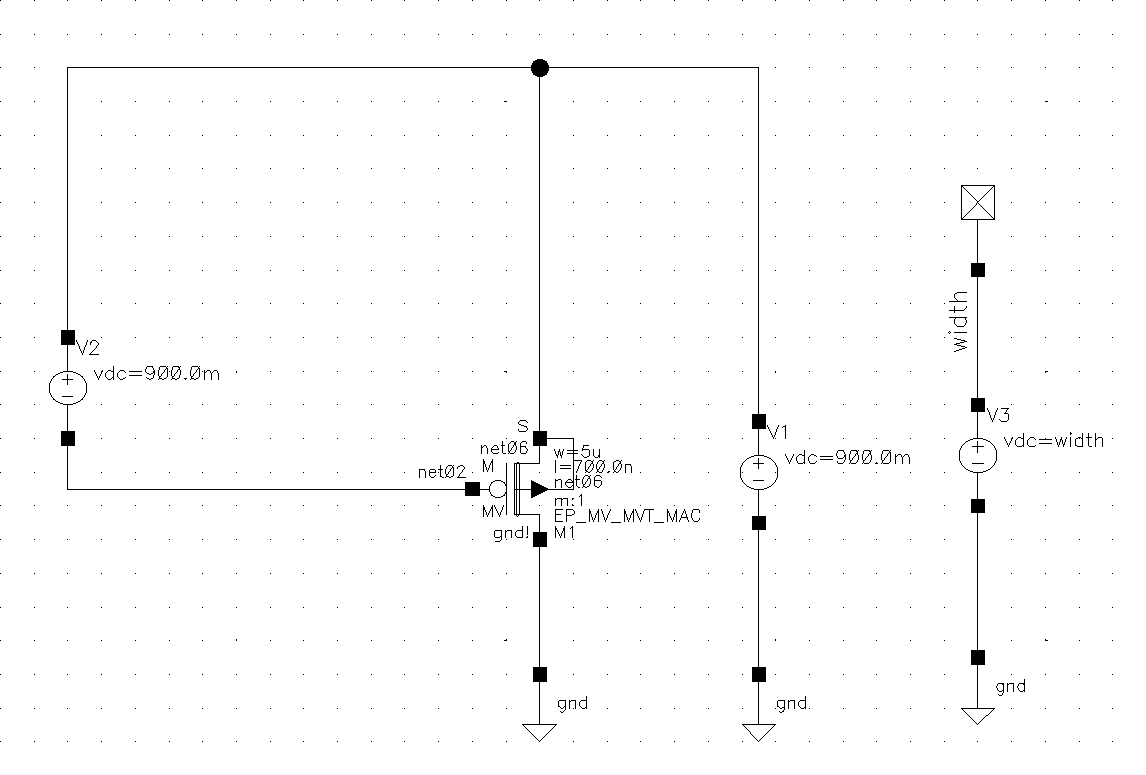
\includegraphics[scale = 0.45]{images/gm_id_pmos_schem.png}
\caption{Schematic of the PMOS transistor setup in cadence}
\label{pmos_setup}
\end{figure}

We then uses $g_m/I_D$ vs $I_D/W$ plot from Fig. \ref{fig:gm_pmos} to obtain the value $I_D/W = 230.137mm$ which corresponds to the $g_m/I_D$ value obtained in equation \ref{gm_ID}. The final width of the transistor is:

\begin{equation}
    W = \frac{I_D}{I_D/W} = 217\mu m
\end{equation}

with the length to the transistor equal to $L = 0.7\mu$, we get:

\begin{equation}
\frac{W}{L} = \frac{217\mu}{0.7\mu} 
\end{equation}


As we will see in the table \ref{final_ota}, this method gives us good accuracy of the desired values needed to satisfy the specifications of the application.


\begin{figure}[ht!]
\begin{subfigure}[c]{0.80\linewidth}
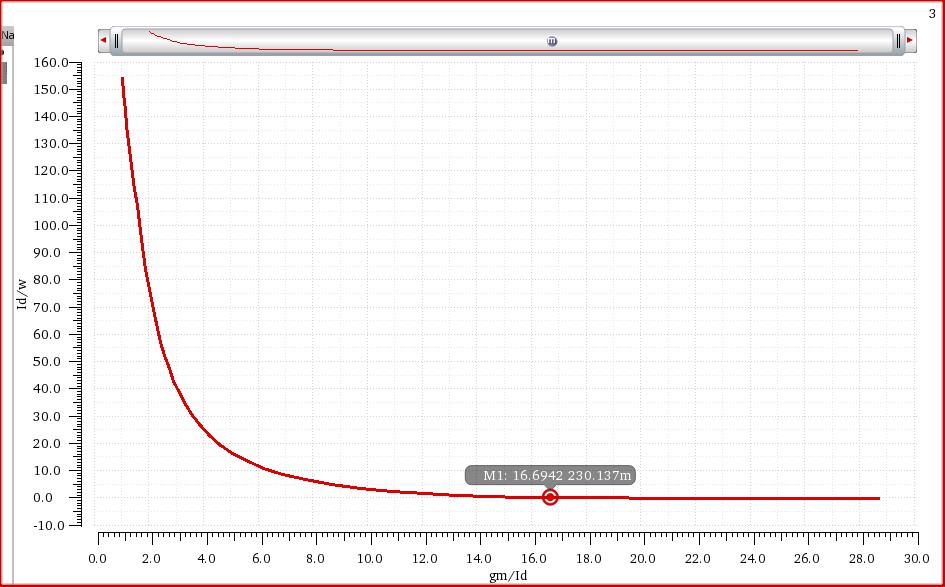
\includegraphics[width = \textwidth]{images/Id_w_vs_gm_id_pmos.jpg}
\caption{PMOS}
\label{fig:gm_pmos}
\end{subfigure}

\begin{subfigure}[c]{0.80\linewidth}
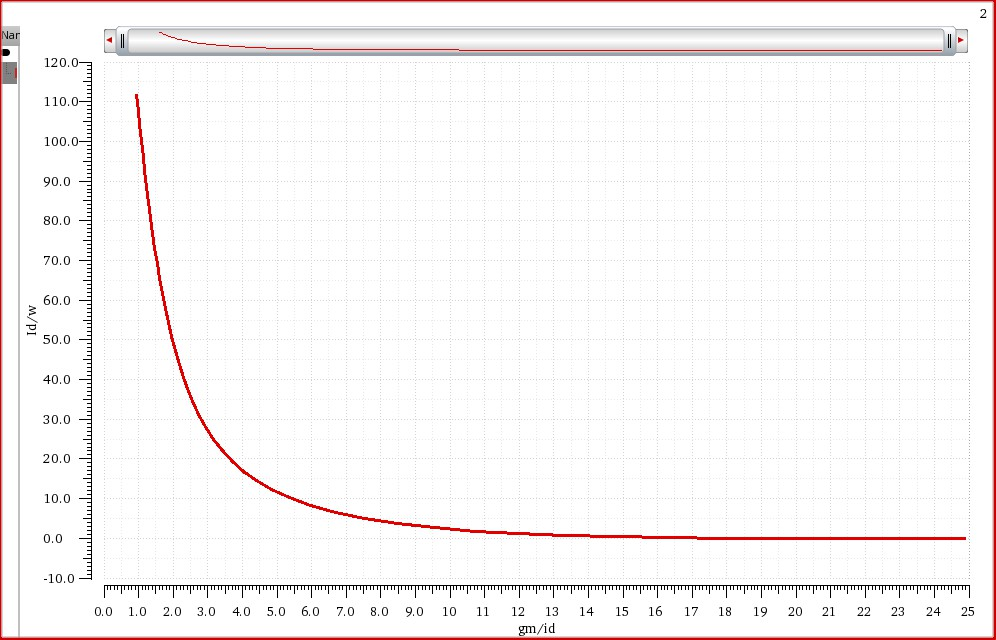
\includegraphics[width = \textwidth]{images/gm_id_w_nmos.jpg}
\caption{NMOS}
\label{fig:gm_nmos}
\end{subfigure}

\caption{Comparison of PMOS and NMOS transistors for $g_m/I_D$ vs $I_D/W$}
\label{fig:comp_pmos_nmos}
\end{figure}


\subsection{Final dimensions of the transistors}

The dimensions for the input transistors of OTA 2 and 3 can be found in a similar manner as it was done for OTA 1 by using table \ref{step_1}, but for transistors $M_3 - M_{11}$ we need to look at the output-swing specification given i table \ref{spec_ota} for the different OTAs. For folded cascode we have a maximum output voltage swing requirement given by\cite{Razavi}:

\begin{equation}
    VO_{max} = V_{DDA} - (V_{OD7} + V_{OD9})
\end{equation}

\begin{equation}
    VO_{min} = V_{OD3} + V_{OD5}
\end{equation}

Where $VO_{max}$ is the upper end and $VO_{min}$ is the lower end of the swing. $V_{OD}$ is the overdrive voltage which define the region the transistor operate in, and is given by the gate voltage and threshold voltage of the transistor:

\begin{equation}
    V_{OD} = V_{GS} - V_{th}
\end{equation}

Since $V_{GS}$ depends on the bias voltage $V_{b}$ we can freely choose which region a transistor will operate in. Transistors in strong inversion has poor current efficiency and low output range, but it is small and the transient frequency is high. Transistors in weak inversion on the other hand has good current efficiency and high output voltage range, but at the cost of a larger transistor and low transient frequency. Moderate inversion is a good compromise between these two regions \cite{gm_id_2}. The goal was to size the transistor to operate as close as possible in this region, thus having good output voltage range while maintaining small area. 

The next step is to use $g_m/I_D$ method to find dimensions for the transistors. The drain current through each transistor can be find using equations: \ref{I_1}, \ref{I_2} and \ref{I_3}. The tranceconductance ($g_m$) of the transistors can be expressed with the help of $V_{OD}$ as follows:

\begin{equation}
    gm = \sqrt{2I_DC_{ox}\frac{W}{L}} = \frac{2I_D}{V_{OD}}
\end{equation}

With the right choice of $V_{OD}$ we can compute the $g_m/I_D$ for a transistor that operate in the moderate inversion region. Then we can use the value of $g_m/I_D$ with the plot in Fig. \ref{fig:gm_pmos} or \ref{fig:gm_nmos} (depending on if we look at PMOS or NMOS transistor) to find the dimension of the transistor, as it was done for transistor $M_1$. This procedure was used as a starting point for sizing the transistors. The final dimensions for the three OTAs were set by using PVT simulations and are summarized in table \ref{final_ota}. The design accomplished the requirements mentioned in table \ref{spec_ota}, as it will be seen in chapter \ref{res:results}.

\begin{table}[h]
\centering
\caption{Transistor dimensions of OTA 1, 2 and 3}
\label{final_ota}
\begin{tabular}{l||l|l||l|l||l|l}
\hline
\multirow{2}{*}{Device} & \multicolumn{2}{c||}{$OTA_1$} & \multicolumn{2}{c||}{$OTA_2$} & \multicolumn{2}{c}{$OTA_3$}\\\cline{2-7}
                        &W[$\mu m$] & L[$\mu m$]& W[$\mu m$] & L[$\mu m$] & W[$\mu m$] & L[$\mu m$]\\\hline
            $M_1$       & 217 & 0.7 & 180 & 0.7 & 163 & 0.7\\
            $M_2$        & 217 & 0.7 & 180 & 0.7 & 163 & 0.7\\
            $M_3$        & 126 & 1 & 97 & 1 & 81 & 1\\
            $M_4$        & 126 & 1 & 97 & 1 & 81 & 1\\
            $M_5$        & 23 & 0.7 & 35 & 0.7 & 25 & 0.7\\
            $M_6$        & 23 & 0.7 & 35 & 0.7 & 25 & 0.7\\
            $M_7$        & 87 & 0.7 & 70 & 0.7 & 52 & 0.7\\
            $M_8$        & 87 & 0.7 & 70 & 0.7 & 52 & 0.7\\
            $M_9$        & 56 & 1 & 43 & 1 & 40 & 1\\
            $M_{10}$        & 56 & 1 & 43 & 1 & 40 & 1\\
            $M_{11}$        & 98 & 1 & 77 & 1 & 66 & 1\\
\hline            
\end{tabular}
\end{table}

\subsection{Bias circuit}

\begin{figure}[h!]
\centering
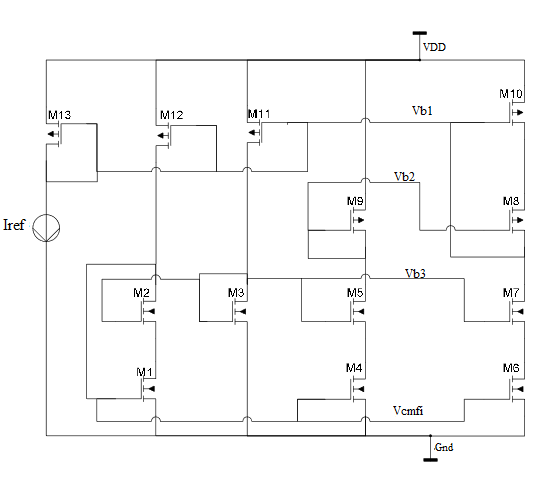
\includegraphics[scale = 0.7]{images/bias_circuit.png}
\caption{Wide swing current mirror}
\label{bias circuit}
\end{figure}

The points $V_{b1}$, $V_{b2}$ and $V_{b3}$ in Fig. \ref{fig:folded_ota_design} is the DC voltages used to bias the transistors, while $V_{cmf}$ controls the common output mode of the OTA. Figure \ref{bias circuit} shows a wide swing current mirror \cite{Allen} which is used to generate the necessary bias voltages in the cascode pair. A wide swing current mirror topology has the perks of not limiting the signal swing as much as the other conventional current mirrors. It also provides a better matching of the currents and higher output resistance. To get a lower power consumption the reference current $I_{ref}$ is set to $10\mu A$, $2\mu A$ and $1\mu A$ for OTA 1, 2 and 3 respectively. With such low currents, especially for OTA 2 and 3, large amounts of noise are generated. This will not be a problem for our ADC, since the noise will be considerably attenuated for OTA 2 and 3. The transistors $M_1-M_3$ and $M_{11}-M_{13}$ are made ten times smaller than the transistors in the cascode of the OTAs. While the dimensions of the transistors $M_{4} - M_{10}$ are the same as the one used in the cascode to make sure that the bias currents listed in table \ref{step_1} are properly mirrored into the OTAs. Transistors $M_3$ and $M_9$ are made four times smaller than transistors $M_2$ and $M_8$ respectively to ensure proper generation of the bias voltages\cite{Johns}. The gate length of the transistors are made to be approximately two times longer than the allowable minimum length to get better matching during layout. Table \ref{final_bias} summarize the transistors dimensions of the circuit for OTA 1, 2 and 3.    

\begin{table}[]
\centering
\caption{Transistor dimensions of the OTAs bias circuits}
\label{final_bias}
\begin{tabular}{l||l|l||l|l||l|l}
\hline
\multirow{2}{*}{Transistor} & \multicolumn{2}{c||}{$OTA_1$} & \multicolumn{2}{c||}{$OTA_2$} & \multicolumn{2}{c}{$OTA_3$}\\\cline{2-7}
                        &W[$\mu m$] & L[$\mu m$]& W[$\mu m$] & L[$\mu m$] & W[$\mu m$] & L[$\mu m$]\\\hline
            $M_1$       & 12.6 & 1 & 9.7 & 1 & 8.1 & 1\\
            $M_2$        & 3.3 & 1 & 5.6 & 1 & 3.6 & 1\\
            $M_3$        & 0.82 & 1 & 1.4 & 1 & 0.9 & 1\\
            $M_4$        & 126 & 1 & 97 & 1 & 81 & 1\\
            $M_5$        & 32.8 & 1 & 56 & 1 & 35.7 & 1\\
            $M_6$        & 126 & 1 & 97 & 1 & 81& 1\\
            $M_7$        & 32.8 & 1 & 56 & 1 & 35.7 & 1\\
            $M_8$        & 124.3 & 1 & 100 & 1 & 74.3 & 1\\
            $M_9$        & 31.1 & 1 & 25 & 1 & 18.6 & 1\\
            $M_{10}$        & 98 & 1 & 77 & 1 & 66 & 1\\
            $M_{11}$        & 9.8 & 1 & 7.7 & 1 & 6.6 & 1\\
            $M_{12}$        & 9.8 & 1 & 7.7 & 1 & 6.6 & 1\\
            $M_{13}$        & 9.8 & 1 & 7.7 & 1 & 6.6 & 1\\
\hline            
\end{tabular}
\end{table}
\clearpage

\subsection{Common mode feedback block}
As mentioned one of the biggest disadvantage of a fully differential OTAs is that, if the common mode output is not controlled it can either go to positive or negative rail and thereby drive some transistors out of the saturation/active region. Hence an additional circuit is required to keep the common mode output stable. Figure \ref{cmfb} shows a switched capacitor common mode feedback block which is a simple circuit used generally in discrete-time circuit. The circuit produce the output common mode voltage by comparing the average of the differential output voltages with the desired common mode voltage. Then the difference between these two voltage ($V_{cmf}$) is used to bring the OTA's common mode voltage back to the desired common mode level. Since the stability of the OTA gets changed when introducing extra capacitors at the output, capacitor $C_1$ and $C_2$ has to be chosen with care. The values were determined by simulation, as a rule of thumb capacitor $C_2$ should be five times larger than $C_1$\cite{Johns}. Table \ref{final_cmfb} list up the capacitance values for OTA 1, 2 and 3. 
\begin{figure}[h!]
\centering
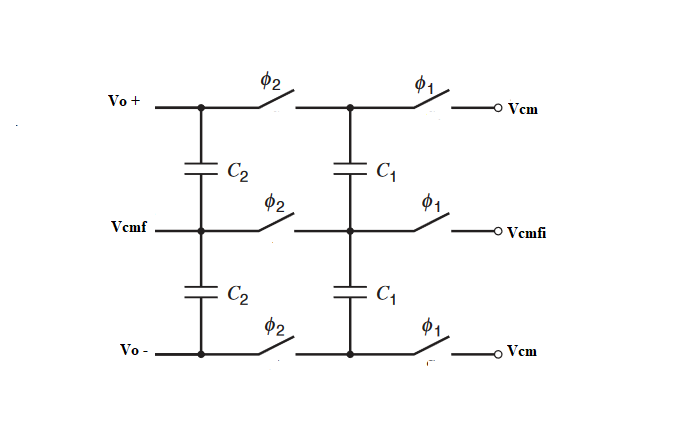
\includegraphics[scale = 0.7]{images/cmf_circuit.png}
\caption{Switched capacitor CMFB circuit\cite{Grey}}
\label{cmfb}
\end{figure}

\begin{table}[h!]
\centering
\caption{CMFB capacitance values}
\label{final_cmfb}
\begin{tabular}{l|l|l|l}
\hline
\multirow{1}{*}{Capacitor} & \multicolumn{1}{c|}{$OTA_1$} & \multicolumn{1}{c|}{$OTA_2$} & \multicolumn{1}{c}{$OTA_3$}\\\cline{1-4}
                       
            $C_1[pF]$       & 1 & 1.35 & 2.1\\
            $C_2 [pF]$      & 0.2 & 0.27 & 0.42 \\
            
\hline            
\end{tabular}
\end{table}

\section{Quantizer}

The quantizer in a $\Delta\Sigma$ ADC has to work at a high oversampling frequency, but its resolution is 1-bit. Therefore we have chosen to implement a latched comparator\cite{comparator} shown in Fig. \ref{quantizer} that focus more on high-speed operation than accuracy. The comparator is clocked in order to synchronize its operation with other circuits in the ADC. The main parameter of concern was  hysteresis, since the input offset and input referred noise get attenuated by the feedback loop of the modulator. 

\begin{figure}[h]
\centering
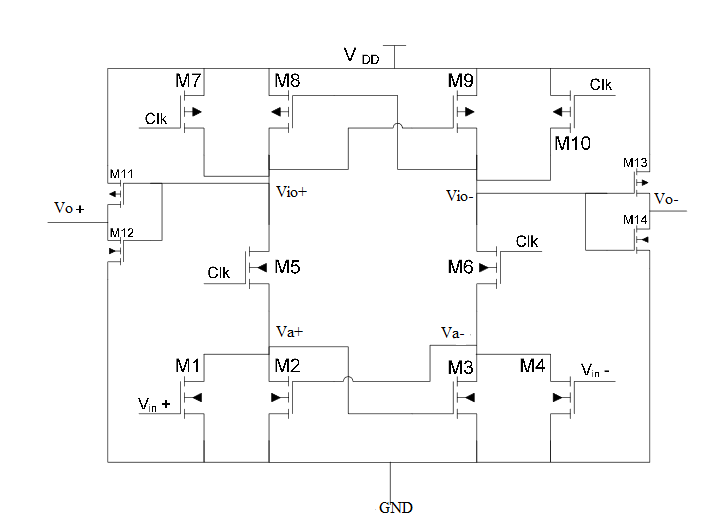
\includegraphics[scale = 0.7]{images/quatizier_circuit.png}
\caption{Latched comparator\cite{comparator}}
\label{quantizer}
\end{figure}

The input $M_1$ and $M_4$ are the discharge controlling transistors which are connected to the flip-flop $M_2$ and $M_3$ in a feedback network. $M_5$ and $M_6$ are control transistors which keep track of holding the comparator synchronized with the rest of the ADC. $M_8$ and $M_9$ are another flip-flop connected in feedback with transistors $M_7$ and $M_{10}$, which are precharge transistors used for refreshing the internal nodes when not in operation to reduce hysteresis. Inverters $M_{11-12}$ and $M_{13-14}$ act as buffers to isolate the latch from the output load and to amplify the comparator output.

When the \textit{Clk} is low, transistors $M_5$ and $M_6$ gets cut off and the input signal will not influence the comparator. The voltages $V_{io+}$ and $V_{io-}$ will be pulled to the positive rail $V_{DD}$, and because of the inverters the output will be pulled to ground. At the same time the voltages $V_a+$ and $V_a-$ gets discharged to ground by transistors $M_1$ and $M_4$. Suppose $V_{in+}$ is greater than $V_{in-}$. When the \textit{Clk} goes high, both voltages $V_{io+}$ and $V_{io-}$ drop from the positive rail and the voltages $V_a+$ and $V_a-$ rise from the ground. However, $M_1$ draws more current than $M_2$, and thereby more current is flowing through $M_3$. This causes $V_{a-}$ to rise faster than $V_{a+}$. Since more current flows through $M_5$ than $M_6$, the voltage $V_{io+}$ drops faster than $V_{io-}$. The regenerative action of $M_8$ and $M_9$ together with that of $M_2$ and $M_3$ pulls $V_{io+}$ to ground and pulls $V_{io-}$ to positive rail. Hence, $V_{0+}$ goes high while $V_{0-}$ goes low. The operation is similar when $V_{in-}$ is greater than $V_{in+}$.

The circuit has digital behaviour with the exception of transistors $M_1$ and $M_4$ that amplify the input signal. Hence, the transistors that operate as digital circuit have minimum dimensions, while the input transistors have a larger length to avoid mismatch effects. The transistor dimensions are listed up in table \ref{final_comparator}.

\begin{table}[]
\centering
\caption{Transistor dimensions of the latched comparator}
\label{final_comparator}
\begin{tabular}{l|l|l}
\hline
\multirow{1}{*}{Transistor} & \multicolumn{1}{c|}{W[$\mu m$]} & \multicolumn{1}{c}{L[$\mu m$]} \\\cline{1-3}
                       
            $M_1$       & 1 & 1\\
            $M_2$      & 0.5 & 0.55\\
            $M_3$      & 0.5 & 0.55\\
            $M_4$      & 1 & 1\\
            $M_5$      & 0.5 & 0.55\\
            $M_6$      & 0.5 & 0.55\\
            $M_7$      & 1 & 0.55\\
            $M_8$      & 1 & 0.55\\
            $M_9$      & 1 & 0.55\\
            $M_{10}$      & 1 & 0.55\\
            $M_{11}$      & 0.5 & 0.55\\
            $M_{12}$      & 0.5 & 0.55\\
            $M_{13}$      & 0.5 & 0.55\\
            $M_{14}$      & 0.5 & 0.55\\
            
\hline            
\end{tabular}
\end{table}

Finally, the output of the comparator is only valid in phase $\phi_1$, and the output of the feedback DAC gets sampled on integrator 1 at phase $\phi_2$. In order to keep the comparator output valid in both phases, a SR-latch is placed in front of the comparator. Since the circuit is purely digital, the dimensions are also here set to minimum. (show figure, either here or appendix?).

\section{Non-overlapping clock generator}
The implemented clock generator is a two-phase non-overlapping circuit. It was designed with the intention of maximize the time available, and make the early and late phases start at the same time, i.e. $\phi_1$ and $\phi_{1d}$ start at the same time. The same apply for phases $\phi_2$ and $\phi_{2d}$. The generator consists of NAND-gates and inverters as shown in Fig. The logic gates have minimum dimensions where the dimensions of the PMOS transistors is three times the NMOS ones. Further delayed clock can be produced by adding more delay inverters on the path from the outputs of the generator to the input of the NOR-gates. Since the switches are transmission gates, each phase needs a complementary singal for proper operation. Complementary signals $\overline{\phi_1}$, $\overline{\phi_{1d}}$, $\overline{\phi_2}$ and $\overline{\phi_{2d}}$ are realized by putting an inverter in front of the outputs of the generator. 

\begin{figure}[h]
\centering
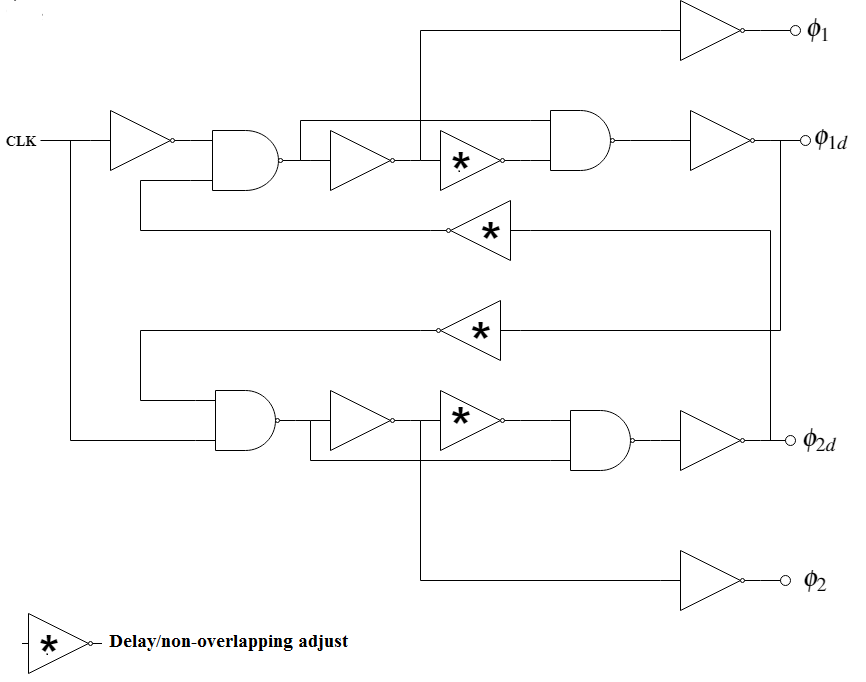
\includegraphics[scale = 0.5]{images/two_phase_clock.png}
\caption{1-bit DAC}
\label{clock_block}
\end{figure}


\section{DAC}
The 1-bit DAC implemented is shown in Fig. \ref{DAC_block}, and the functionality is simple. For instance, depending on if the input signal dacp\_1 is either high or low the feedback out back to integrator 1 is either vrefp or vrefn which is the reference voltages. Similarly the output vfbp depends on the level of input dacn\_1. In a differential circuit, the reference voltages must be centered at the analog ground $V_{cm} = 0.9V$. Hence, they have to be implemented so they are symmetric with respect to $V_{cm}$ such that their difference is equal to $V_{ref}$ (listed in table \ref{spec}). The reference voltages are chosen to be $\pm 0.5$ around $V_{cm}$. Therefore, vrefp is 1.4V and vrefn is 0.4V. The switches is implemented as TG switch with the dimensions of PMOS switch being $\frac{W}{L}_p = \frac{10.5}{0.55}\mu m$ and $\frac{W}{L}_n = \frac{3.5}{0.55}\mu m$, giving an on-resistance of $905.4\Omega$. 

\begin{figure}[]
\centering
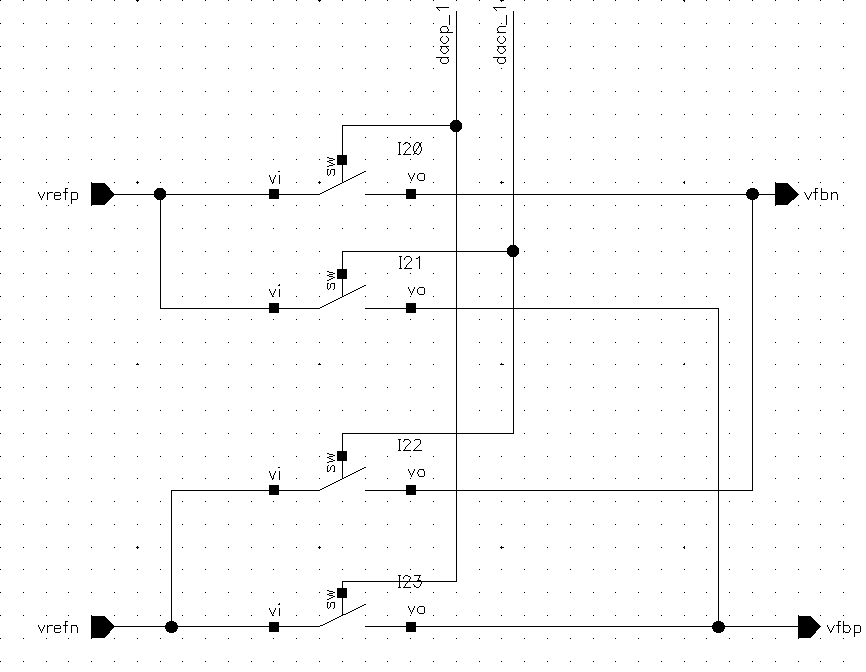
\includegraphics[scale = 0.45]{images/DAC_block.png}
\caption{1-bit DAC}
\label{DAC_block}
\end{figure}